\documentclass[conference,a4paper]{IEEEtran}

% added package by asfihani
\usepackage{url}
\usepackage{graphicx}
\usepackage{algorithm}
\usepackage{algpseudocode}
\usepackage{multirow}
\usepackage{booktabs}
\usepackage{stfloats}
% correct bad hyphenation here
\hyphenation{op-tical net-works semi-conduc-tor parti-cipant techno-logy}

\DeclareRobustCommand*{\IEEEauthorrefmark}[1]{\raisebox{0pt}[0pt][0pt]{\textsuperscript{\footnotesize #1}}}

\begin{document}
\title{User Study of Palm Gesture Recognition Tracking Human-Computer Interaction System Based on PAJ7620 Motion Sensor}

\author{\IEEEauthorblockN{Asfihani\IEEEauthorrefmark{1} and Hadziq Fabroyir\IEEEauthorrefmark{2}}           

\\
\IEEEauthorblockA{\IEEEauthorrefmark{1,2}
Department of Informatics, The Faculty of Intelligent Electrical and Informatics Technology,\\
Institut Teknologi Sepuluh Nopember, Surabaya, East Java, Indonesia.}\\

\textsuperscript{1}6025231054@student.its.ac.id, \textsuperscript{2}hadziq@its.ac.id
}

\maketitle
\begin{abstract}
In recent years, the field of human-computer interaction has witnessed a growing demand for natural and intuitive interfaces that enable seamless communication between humans and machines. Palm gesture recognition has emerged as a promising approach for this enablement, as it allowed users to interact with computers and devices through gestures and movements, mimicking real-world interactions. This research presents the implementation and user study of a palm gesture recognition tracking human-computer intelligent interaction system based on the PAJ7620 gesture using controller on Spotify streaming application. The research indicates that the use of palm gestures recognition for the Spotify application to control playback has not shown positive results.
\end{abstract}
{\smallskip \keywords Palm Gesture Recognition, Human-Computer Interaction, Spotify, Arduino Uno, PAJ7620 Sensor.}

\IEEEpeerreviewmaketitle

\vspace{7pt}
\section{Introduction}
Palm gesture recognition was a cutting-edge technology that has gained significant prominence. It involved the interpretation and understanding of human hand movements and gestures through the use of computational algorithms and advanced sensors. This field had applications in various domains, ranging from human-computer interaction to robotics, virtual reality, sign language recognition, and more. The primary objective of palm gesture recognition was to bridge the gap between human communication and digital interfaces, allowing for more intuitive and natural interactions with machines and devices. By capturing and deciphering the intricate movements of the palm, computers could interpret gestures as commands, enabling users to control and manipulate technology effortlessly.

Gesture recognition technology was a hot research topic in human-computer interaction because it was intuitive, vivid, and visually appealing. This technology uses image processing, pattern recognition, and computer vision to analyze palm movements captured by a camera or sensor and recognize them as commands  \cite{vidyagesture}. These commands could control computer functions for media players like Spotify, Netflix, and YouTube. Gesture technology could also control electronic devices, such as the Microsoft Xbox 360, Nintendo Wii, Nintendo Switch, and many smart TVs, by shaking a body part to perform specific tasks. In other words, gesture recognition technology allows people to interact with computers and other devices using their hands and body movements rather than a keyboard and mouse. This technology was still under development, but it has the potential to revolutionize the way we interact with technology.

This study aimed to develop a method to control the Spotify application on a computer using a PAJ7620 sensor connected to an Arduino Uno microcontroller. The PAJ7620 sensor could detect nine types of movements: up, down, left, right, forward, backward, clockwise, counterclockwise, and rocking (waving) \cite{pixart} \cite{taufikproto}. The PAJ7620 sensor captured motion from palm gestures and then converts it into data, which was sent to the Arduino Uno microcontroller using a serial port. A Python program will monitor the data from the serial port and then trigger an event based on the predefined pattern of the palm gesture. The final result was the ability to control the Spotify application, such as playing the next track, the previous track, increasing the volume, decreasing the volume, starting or stopping the music, pausing or resuming the music, replaying the track, and toggling shuffle on or off.

%\begin{figure}
%    \centering
%    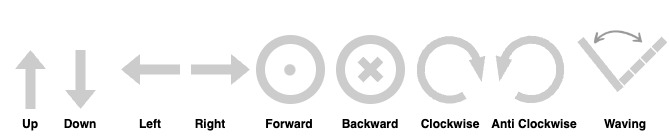
\includegraphics[width=0.75\linewidth]{movement.jpg}
%    \caption{Nine Gestures Recognition}
%    \label{fig:nine-movements}
%\end{figure}

\vspace{7pt}
\section{Related Work}
The research by \cite{rahmifountain} created a system that uses a PAJ7620 sensor and Arduino Uno to capture and process hand gestures, which are then used to control the burst pattern of a fountain. The research by \cite{SHARMA2015721} explores the importance of input approaches in contemporary technology, underscoring the utilization of touchless methods such as hand gestures and speech for computer applications. It underscores the potential advantages of hand gesture control, especially for individuals with physical challenges, while recognizing the imperative to enhance the reliability of gesture recognition and detection. Additionally, it contemplates the potential extension of the system to manage a diverse range of applications.

The research by \cite{jianweiwheel} on intelligent IoT wheelchairs enhanced with PAJ7620 for gesture recognition and GPS and IMU sensors for positioning and posture aims to improve traditional wheelchairs. These advanced wheelchairs offer increased intelligence, versatility, and safety. However, they grapple with issues like cluttered wiring and vulnerable components, underscoring the importance of design refinements, especially concerning slope safety. The study by  \cite{jenlicar} on car parking sensors by measuring the distance controller using ultrasonic sensors based on Arduino Uno, Arduino MP3 Shield, and Ultrasonic HC-SR04, which aim to help the driver. The research aims to measure the car's distance from the object behind it to help the driver determine the safe distance to park their car. 

The study by \cite{wangthree} of human-computer interaction system research utilized the PAJ7620 motion sensor and STM32 chip to accurately recognize and display 3D gesture information on an OLED screen. Experiments revealed near-perfect gesture recognition within 10 cm, with accuracy declining after 10 cm and dropping significantly beyond 25 cm. Future work should concentrate on improving the gesture recognition algorithm and enhancing accuracy in complex settings. The research by  \cite{dhamanskar} on human-computer interaction on hand gestures and voice using deep learning machine and image recognition. A gesture recognition and hand tracking system was developed to allow users to interact with PC applications using hand gestures, eliminating the need for a mouse and keyboard. This intuitive system can be calibrated for various skin colors and backgrounds and recognizes real-time gestures like clicks. Additionally, it features voice command integration for an even more straightforward user experience. 

The research conducted by \cite{jhuuwb} explored an affordable system that employs ultra-wideband (UWB) radar to identify eye blinks, all without the need for cameras, sound-based techniques, or specialized equipment. BlinkRadar proves capable of consistently spotting driver blinks in real-world driving scenarios, allowing for the detection of drowsy driving incidents. The authors utilized the multi-sequence variational mode decomposition (MS-VMD) algorithm to separate the eye blink signal from background noise. Thorough experimentation in two distinct settings demonstrated that BlinkRadar achieves an impressive average blink detection accuracy of more than 96.2\%.

\vspace{7pt}
\section{Architecture}
The illustration in Fig. \ref{fig:system-design} provides an overview of the system's overall structure and constituent parts. These components include the PAJ7620 sensor, which was responsible for detecting palm gestures; the Arduino Uno, which functions as a microcontroller to handle sensor data and transmit it to the serial port; and a computer running the Spotify application on a macOS Sonoma (14.0) serving as the recipient of this serial data.

\begin{figure}[!tbh]
    \centering
    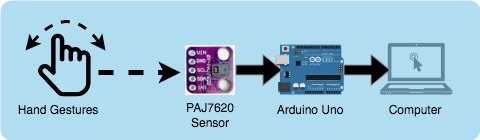
\includegraphics[width=0.9\linewidth]{system-design.png}
    \caption{System Design}
    \label{fig:system-design}
\end{figure}

In this study, the resulting output was determined by analyzing eight distinct palm gesture patterns recorded by the sensor. Each pattern corresponds to a unique action, which the details can be found in TABLE \ref{table1}.

\begin{table}[!tbh]
  \centering
  \footnotesize % \onehalfspacing
  \caption{Pattern and Action}
  \begin{tabular}{p{0.3cm}p{1.65cm}p{3.4cm}p{2.25cm}}
     \toprule
     \normalfont Patt. & Gesture & Description & Action \\
     \midrule
      1 & right & palm to the right & next track\\ 
      2 & left & palm to the left & previous track\\ 
      3 & up & palm up& increase the volume\\ 
      4 & down & palm down& reduce the volume\\ 
      5 & forward & palm towards the sensor & stop/pause\\ 
      6 & backward& palm away from the sensor & start/resume\\  
      7 & clockwise& fingers rotated clockwise & replay track\\ 
      8 & anti-clockwise& fingers rotated anti-clockwise& shuffle on/off\\
     \bottomrule
  \end{tabular}
  \label{table1}
\end{table}

\subsection{Pattern 1}
The palm was moved from the left to the right in front of the sensor as shown in Fig. \ref{fig:pattern-1}. The expected result was that the sensor captures the movement and specific data passed to the microcontroller. The computer will read data from a serial port and translate it to instruction as the next track.

\begin{figure}[!h]
    \centering
    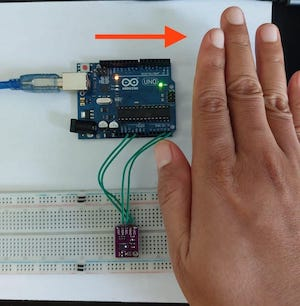
\includegraphics[width=0.5\linewidth]{hand-right.jpeg}
    \caption{Pattern 1}
    \label{fig:pattern-1}
\end{figure}

\subsection{Pattern 2}
The palm was moved from the right to the left in front of the sensor as shown in Fig. \ref{fig:pattern-2}. The expected result was that the sensor captures the movement and specific data passed to the microcontroller. The computer will read data from a serial port and translate it to instructions as the previous track.

\begin{figure}[!h]
    \centering
    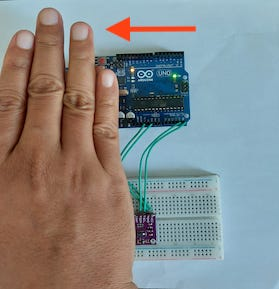
\includegraphics[width=0.5\linewidth]{hand-left.jpeg}
    \caption{Pattern 2}
    \label{fig:pattern-2}
\end{figure}

\subsection{Pattern 3}
The palm was moved from the bottom to the top in front of the sensor as shown in Fig. \ref{fig:pattern-3}. The expected result was that the sensor captures the movement and specific data passed to the microcontroller. The computer will read data from a serial port and translate it to instructions to increase the volume.

\begin{figure}[!h]
    \centering
    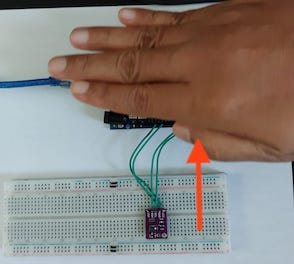
\includegraphics[width=0.5\linewidth]{hand-up.jpeg}
    \caption{Pattern 3}
    \label{fig:pattern-3}
\end{figure}

\subsection{Pattern 4}
The palm was moved from up to the bottom in front of the sensor as shown in Fig. \ref{fig:pattern-4}. The expected result was that the sensor captures the movement and specific data passed to the microcontroller. The computer will read data from a serial port and translate it to instructions to reduce the volume.

\begin{figure}[!h]
    \centering
    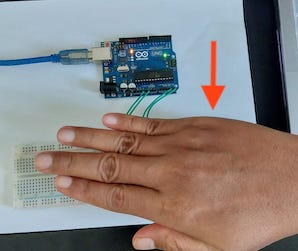
\includegraphics[width=0.5\linewidth]{hand-down.jpeg}
    \caption{Pattern 4}
    \label{fig:pattern-4}
\end{figure}

\subsection{Pattern 5}
The palm was moved towards the sensor as shown in Fig. \ref{fig:pattern-5}. The expected result was that the sensor captures the movement and specific data passed to the microcontroller. The computer will read data from a serial port and translate it to instructions to stop/pause the track.

\begin{figure}[!h]
    \centering
    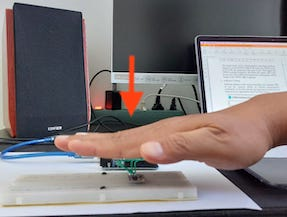
\includegraphics[width=0.5\linewidth]{hand-forward.jpeg}
    \caption{Pattern 5}
    \label{fig:pattern-5}
\end{figure}

\subsection{Pattern 6}
The palm was moved away from the sensor as shown in Fig. \ref{fig:pattern-6}. The expected result was that the sensor captures the movement and specific data passed to the microcontroller. The computer will read data from a serial port and translate it to instructions to start/resume the track.

\begin{figure}[!h]
    \centering
    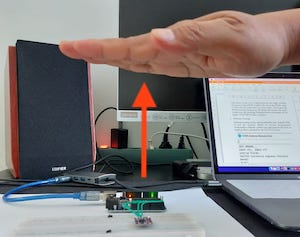
\includegraphics[width=0.5\linewidth]{hand-backward.jpeg}
    \caption{Pattern 6}
    \label{fig:pattern-6}
\end{figure}

\subsection{Pattern 7}
The fingers are rotated clockwise was front of the sensor in this pattern  as shown in Fig. \ref{fig:pattern-7}. The expected result was that the sensor captures the movement and specific data passed to the microcontroller. The computer will read data from a serial port and translate it to instructions to replay the current track.

\begin{figure}[!h]
    \centering
    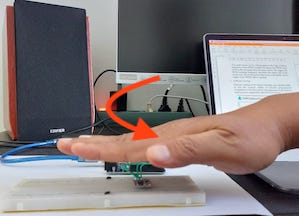
\includegraphics[width=0.5\linewidth]{hand-clockwise.jpeg}
    \caption{Pattern 7}
    \label{fig:pattern-7}
\end{figure}

\subsection{Pattern 8}
The fingers are rotated anti-clockwise in front of the sensor in this pattern  as shown in Fig. \ref{fig:pattern-8}. The expected result was that the sensor captures the movement and specific data passed to the microcontroller. The computer will read data from a serial port and translate it to instructions to replay the toggle shuffle on or off.

\begin{figure}[!h]
    \centering
    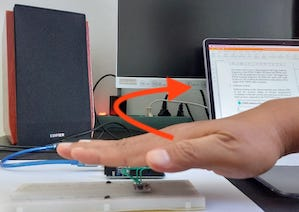
\includegraphics[width=0.5\linewidth]{hand-anti-clockwise.jpeg}
    \caption{Pattern 8}
    \label{fig:pattern-8}
\end{figure}

The hardware configuration depicted in Fig. \ref{fig:hardware-design} comprised input, processing, and output components. The input includes a palm gesture and a PAJ7620 sensor, which is responsible for detecting and interpreting palm gestures. Subsequently, the data is transmitted to the Arduino Uno microcontroller through the Python and Spotify program. Finally, the processed data was forwarded to the output, involving a speaker and the Spotify application on a computer.

\begin{figure}[tbh!]
    \centering
    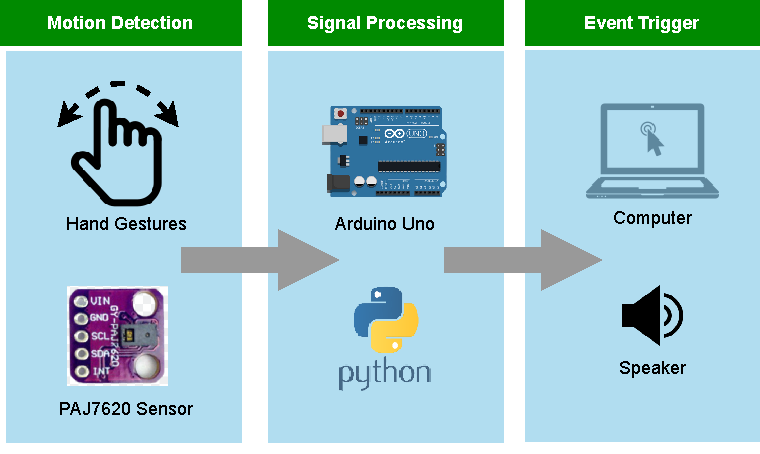
\includegraphics[width=0.9\linewidth]{hardware-design.pdf}
    \caption{Hardware Design}
    \label{fig:hardware-design}
\end{figure}

The software design of the system was the program flow that will run on the Arduino Uno microcontroller, which then pass specific data to the serial port where the computer which runs a Python program with the help of shpotify\footnote{\url{https://github.com/hnarayanan/shpotify}} --- a Spotify command line client for Mac OS --- to control the Spotify application. The system identified palm gestures captured by the PAJ7620 sensor and determined which value was being passed to the Python program, triggering a predefined function based on that data. 

\section{Testing and Analysis}
The research involved a three-step process consisting of hardware testing, software testing, and system testing. These evaluations aimed to ascertain the system's capability to interpret user actions based on palm gestures as input, assessing the effectiveness of the designed system.

\subsection{Hardware Testing}
Hardware testing was conducted on the PAJ7620 sensor to ascertain its ability to detect and accurately transmit data to the Arduino Uno microcontroller when encountering various foreign objects. The experiment used multiple objects, and the outcomes are detailed in TABLE \ref{table2}. The physical hardware setup is illustrated in Fig. \ref{fig:hardware-setup}.

\begin{table}[hbt!]
\centering
  \footnotesize % \onehalfspacing
  \caption{Object Detection Test on PAJ7620 Sensor}
  \begin{tabular}{p{0.5cm}p{3cm}p{1.5cm}}
     \toprule
     \normalfont No.& Object& Result\\
     \midrule
      1 & front palm of the hand& detected\\ 
      2 & back palm of the hand& detected\\
      3 & fingers& detected\\  
      4 & spoon& detected\\ 
      5 & paper& detected\\  
      6 & wood& detected\\ 
      7 & solid plastic& detected\\
      8 & grocery plastic bag& detected\\
     \bottomrule
  \end{tabular}
  \label{table2}
\end{table}

\begin{figure}[hbt!]
    \centering
    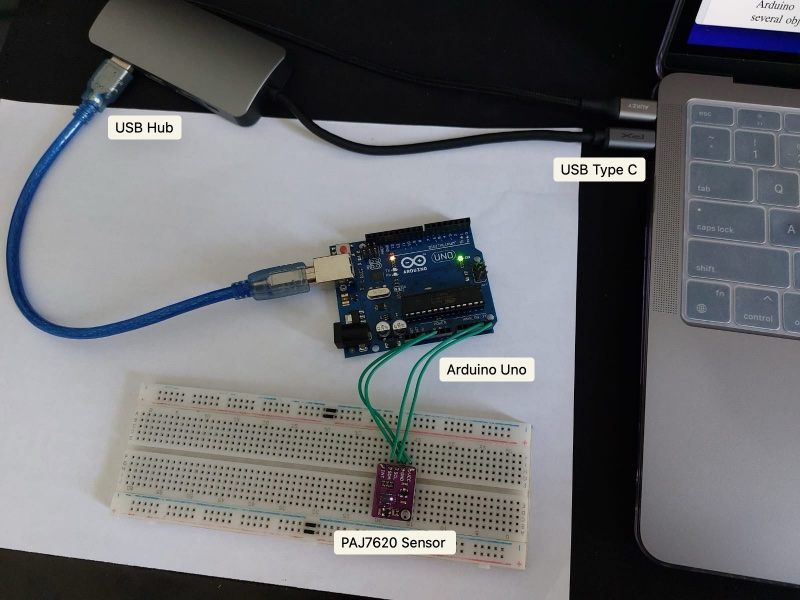
\includegraphics[width=0.75\linewidth]{hardware-setup.jpeg}
    \caption{Hardware Setup}
    \label{fig:hardware-setup}
\end{figure}

\subsection{Software Testing}
The microcontroller undergoes software testing through Arduino IDE to assess its capacity to receive data from the PAJ7620 sensor via the serial port. As a result, the Arduino microcontroller can identify palm gestures made by the user, transmitting this data to the computer. Subsequently, a Python script monitors the serial port, prompting the execution of specific events in the Spotify program by predefined patterns.

\subsection{System Testing}

The diagram illustrating the system testing configuration can be seen in Fig. \ref{fig:system-testing-setup}. In this experiment, participants were instructed to glide their palms over a sensor connected to the Arduino Uno board, which was linked to a computer running Spotify. The objective of this testing was to assess the PAJ7620 sensor's ability to detect and interpret palm gestures. These hand movements included eight distinct gestures: moving the palm to the right, left, up, down, forward, backward, clockwise, and anti-clockwise. The palm was initially positioned directly on the top of the sensor camera and then moved in the intended direction. We conducted 10 trials for each predefined gesture, varying the distance from the sensor at 10cm, 20cm, 25cm, and 30cm.

\begin{figure}[hbt!]
    \centering
    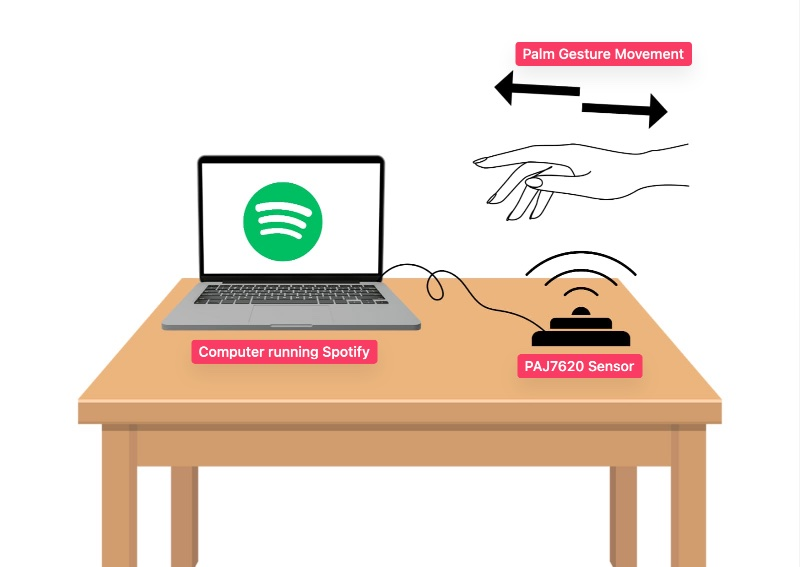
\includegraphics[width=0.85\linewidth]{system-testing.jpeg}
    \caption{System Testing Setup}
    \label{fig:system-testing-setup}
\end{figure}


\subsection{User Study}
To verify the system's performance, we recruited 5 participants, two males and three females aged 25 to 45, with various jobs as housewives, self-employed, students, and housekeepers. We conducted a study to assess how different factors affect the operational range of the PAJ7620 sensor. This evaluation aimed to determine if the Spotify application can successfully execute tasks using palm gesture inputs provided by the user's patterns.

Based on the tests we carried out, as in TABLE \ref{table3}, the Spotify application can act according to the hand gesture inputted by the user. In our test, the success rate of right, left, backward, and forward gestures can reach around 100\%. The success rate for up, down, clockwise, and anti-clockwise gesture are around 80\%-90\%. The PAJ7620 sensor works best in distances 5cm - 25cm and cannot capture the gesture when the distance exceeds 25cm.

\begin{table}[hbt!]
\centering
\caption{Success Rate of Gestures}
\begin{tabular}{lllll}
\toprule
\multirow{2}{*}{Pattern} & \multicolumn{4}{c}{Distance}                                                          \\ \cmidrule(r){2-5} 
                         & \multicolumn{1}{l}{10 cm}    & \multicolumn{1}{l}{20 cm}    & \multicolumn{1}{l}{25 cm}    & 30 cm\\   
\midrule
Right                    & \multicolumn{1}{l}{10/10} & \multicolumn{1}{l}{10/10} & \multicolumn{1}{l}{10/10} & 0/10 \\
Left                     & \multicolumn{1}{l}{10/10} & \multicolumn{1}{l}{10/10} & \multicolumn{1}{l}{10/10} & 0/10 \\
Up                       & \multicolumn{1}{l}{10/10} & \multicolumn{1}{l}{10/10} & \multicolumn{1}{l}{10/10} & 0/10 \\
Down                     & \multicolumn{1}{l}{10/10} & \multicolumn{1}{l}{10/10} & \multicolumn{1}{l}{10/10} & 0/10 \\
Forward                  & \multicolumn{1}{l}{10/10} & \multicolumn{1}{l}{10/10} & \multicolumn{1}{l}{5/10} & 0/10 \\
Backward                 & \multicolumn{1}{l}{10/10} & \multicolumn{1}{l}{10/10} & \multicolumn{1}{l}{5/10} & 0/10 \\
Clockwise                & \multicolumn{1}{l}{10/10} & \multicolumn{1}{l}{10/10} & \multicolumn{1}{l}{7/10} & 0/10 \\
Anti-clockwise           & \multicolumn{1}{l}{10/10} & \multicolumn{1}{l}{10/10} & \multicolumn{1}{l}{7/10} & 0/10 \\ 
\bottomrule
\end{tabular}
\label{table3}
\end{table}

We also compared the total completion tasks for each participant to complete the task based on existing system (A) and proposed system (B) which the result can be shown in the TABLE \ref{table4}. We found that the user experience was not satisfied compared to existing systems, due the time required to operate the proposed system exceeds the existing time of the existing system.

\begin{table}[!h]
\centering
\caption{Completion time}
\begin{tabular}{lll}
\toprule
\multirow{2}{*}{Participant} & \multicolumn{2}{l}{Method} \\
\cmidrule(r){2-3} 
& A & B \\ 
\midrule
1 &	5 &	10 \\
2 &	8 &	13 \\
3 &	7 &	9 \\
4 &	5 &	11 \\
5 &	6 &	14 \\
\midrule
Avg. Mean &	\textbf{6.2} & 11.4 \\
Std. Dev. & \textbf{1.3} & 2.1 \\
\bottomrule
\end{tabular}
\label{table4}
\end{table}

The Fig. \ref{fig:completion-time} show the average mean comparasion to complete the tasks between existing system (A) and proposed system (B).

\begin{figure}[hbt!]
    \centering
    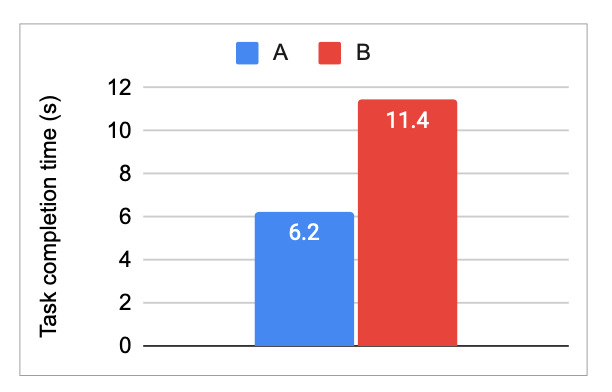
\includegraphics[width=0.85\linewidth]{completion-time.png}
    \caption{Average Completion Time}
    \label{fig:completion-time}
\end{figure}

\section{Conclusion}
The Spotify application can act according to the hand gesture input from the user. In our test, the success rate of right, left, backward, and forward gestures can reach around 100\%. The success rate for up, down, clockwise, and anti-clockwise gestures is around 80\%-90\%. Our test also found that the best distance when conducting the tests is around 5cm - 25cm, and the PAJ7620 sensor should be placed on a flat surface. However the user experience was not good compared to existing system due to the completion time problem. In the future, this system can be improved by controlling the media player using a predefined keyboard function such as Python PyAutoGUI\footnote{https://pyautogui.readthedocs.io/} instead of relying on one specific program,  to manage all media players, such as Netflix, YouTube, VLC, and Apple Music.

\vspace{7pt}
\begin{thebibliography}{1}

\bibitem{vidyagesture}
M. Vidya, S. Vineela, P. Sathish and A. S. Reddy, \emph{"Gesture-Based Control of Presentation Slides using OpenCV"}, 2023 Second International Conference on Augmented Intelligence and Sustainable Systems (ICAISS), Trichy, India, 2023, pp. 1786-1791, doi: 10.1109/ICAISS58487.2023.10250520.

\bibitem{pixart}
PixArt Imaging Inc., \emph{"PAJ7620F2: Integrated Gesture Recognition Sensor"}, \url{https://www.epsglobal.com/Media-Library/EPSGlobal/Products/files/pixart/PAJ7620F2.pdf}, 
2016, Accessed: 2023-10-08.

\bibitem{taufikproto}
T. A. Wibowo and R. E Putri, \emph{"Prototype of Smart Minimarket"}, JITCE (Journal of Information Technology and Computer Engineering), vol. 3(01), pp. 39-53, 2019, doi: 10.25077/jitce.3.01.39-53.2019.

\bibitem{rahmifountain}
R. E. Putri and N. A. S. Nazara, \emph{"The Implementation Of Hand Gestures On The Fountain Burst Pattern"}, 2022 International Symposium on Information Technology and Digital Innovation (ISITDI), Padang, Indonesia, 2022, pp. 27-31, doi: 10.1109/ISITDI55734.2022.9944432.

\bibitem{SHARMA2015721}
R. P. Sharma and Gyanendra K. Verma, \emph{"Human Computer Interaction using Hand Gesture"}, Procedia Computer Science, Volume 54, 2015, Pages 721-727, ISSN 1877-0509, doi: 10.1016/j.procs.2015.06.085.

\bibitem{jianweiwheel}
Cui J., Cui L., Huang Z., Li X., and Han F., \emph{"IoT Wheelchair Control System Based on Multi-Mode Sensing and Human-Machine Interaction"}, Micromachines, 2022; vol. 13(7), pp. 1108, doi: 10.3390/mi13071108.
  
\bibitem{jenlicar}
J. Susilo, A. Febriani, U. Rahmalisa, and Y. Irawan, \emph{"Car Parking Distance Controller Using Ultrasonic Sensors Based On Arduino Uno"}, Journal of Robotics and Control (JRC), 2021, vol. 2 (5), pp: 353-356, doi: 10.18196/jrc.25106. 

\bibitem{wangthree}
W. Jian-liang, W. Ye, L. Yang, et al.,\emph{"Design of Three-Dimensional Gesture Recognition and Motion Tracking Human-Computer Intelligent Interaction System based on PAJ7620"}, 2021 International Conference on Information Technology, 2021, vol. 2005, doi: 10.1088/1742-6596/2005/1/012085.

\bibitem{dhamanskar}
P. Dhamanskar, A. C. Poojari, H. S. Sarwade and R. R. D'silva, \emph{"Human Computer Interaction using Hand Gestures and Voice"}, 2019 International Conference on Advances in Computing, Communication and Control (ICAC3), Mumbai, India, 2019, pp. 1-6, doi: 10.1109/ICAC347590.2019.9036817.

\bibitem{jhuuwb}
J. Hu, J. Hongbo, L. Daibo, Z. Qibo, M.Geyong, and L. Jiangchuanm, \emph{"Real-Time Contactless Eye Blink Detection Using UWB Radar"}, IEEE Transactions on Mobile Computing, Oct 2023, pp. 1-4, doi: 10.1109/TMC.2023.3323280.

\end{thebibliography}
% that's all folks
\end{document}



